\documentclass[12pt, oneside, a4paper]{article}

% for math symbols
\usepackage{amsmath}
\usepackage{amssymb}
% for inserting images
\usepackage{graphicx}
% for algorithm pseudocode
\usepackage{algorithm}
\usepackage{algpseudocode}
% for tables
\usepackage{tabularx}
% for implementation of the array and tabular environments
\usepackage{array}
% Control float placement. Defines a \FloatBarrier command
\usepackage{placeins}
% for derivative commands
\usepackage{physics}
% for multi level lists
\usepackage{outlines} 
% for links in text
\usepackage[colorlinks=true,linkcolor=blue,urlcolor=black,bookmarksopen=true]{hyperref}
% for contents after pdf is formed
\usepackage{bookmark}
% for caption
\usepackage{caption}
% for code
\usepackage{listings}
% for pictures
\usepackage{tikz}


\def\nudge{.5}
\tikzset{axis/.style={ultra thick, black, -latex, shorten <=-\nudge cm, shorten >=-2*\nudge cm}}
\tikzset{line/.style={thick,green}}

\hypersetup{%
  colorlinks=true,
  linkcolor=blue,
  linkbordercolor={0 0 1}
}

\newcommand{\vect}[1]{\ensuremath{\mathbf{#1}}}
\newcommand{\vt}[1]{\ensuremath{\mathbf{#1}}}
\newcommand{\uline}[1]{\underline{#1}}
\newcommand{\tb}[1]{\textbf{#1}}

\DeclareUnicodeCharacter{2212}{\textendash}

\graphicspath{ {./images/} }

\title{CSDS 341: Final Project Initial Report\\ Questionnaire Website}
\author{Oleksii Fedorenko, David Frost, Matthew Garcia, Preeti Naik}

\begin{document} 
    \maketitle
    \section{Background}
    Questionnaires and surveys are very important for understanding and shaping the world. Surveys are one of the main tools for collection and analysis of data for making decisions. For example, United States uses the Census and the American Community Survey to understand how the country's demographics are shifting and to make decisions about the allocation of resources. Researchers use questionnaires for scientific studies to understand both the social and natural worlds. Psychologists in particular make great use of Likert scales in questionnaires to help build our collective knowledge.   
    
    Therefore, streamlining the process of collecting and analysing surveys using technology is very beneficial for decision-making. Our application would allow users to create their own questionnaires, distribute and analyse them easily. Additionally, application would allow for streamlining the decision-making process based on the analysis of data to an advanced degree.
    

    \newpage    
    \section{ER Diagram}  

    \FloatBarrier
    \begin{figure}[H] 
        \centerline{
        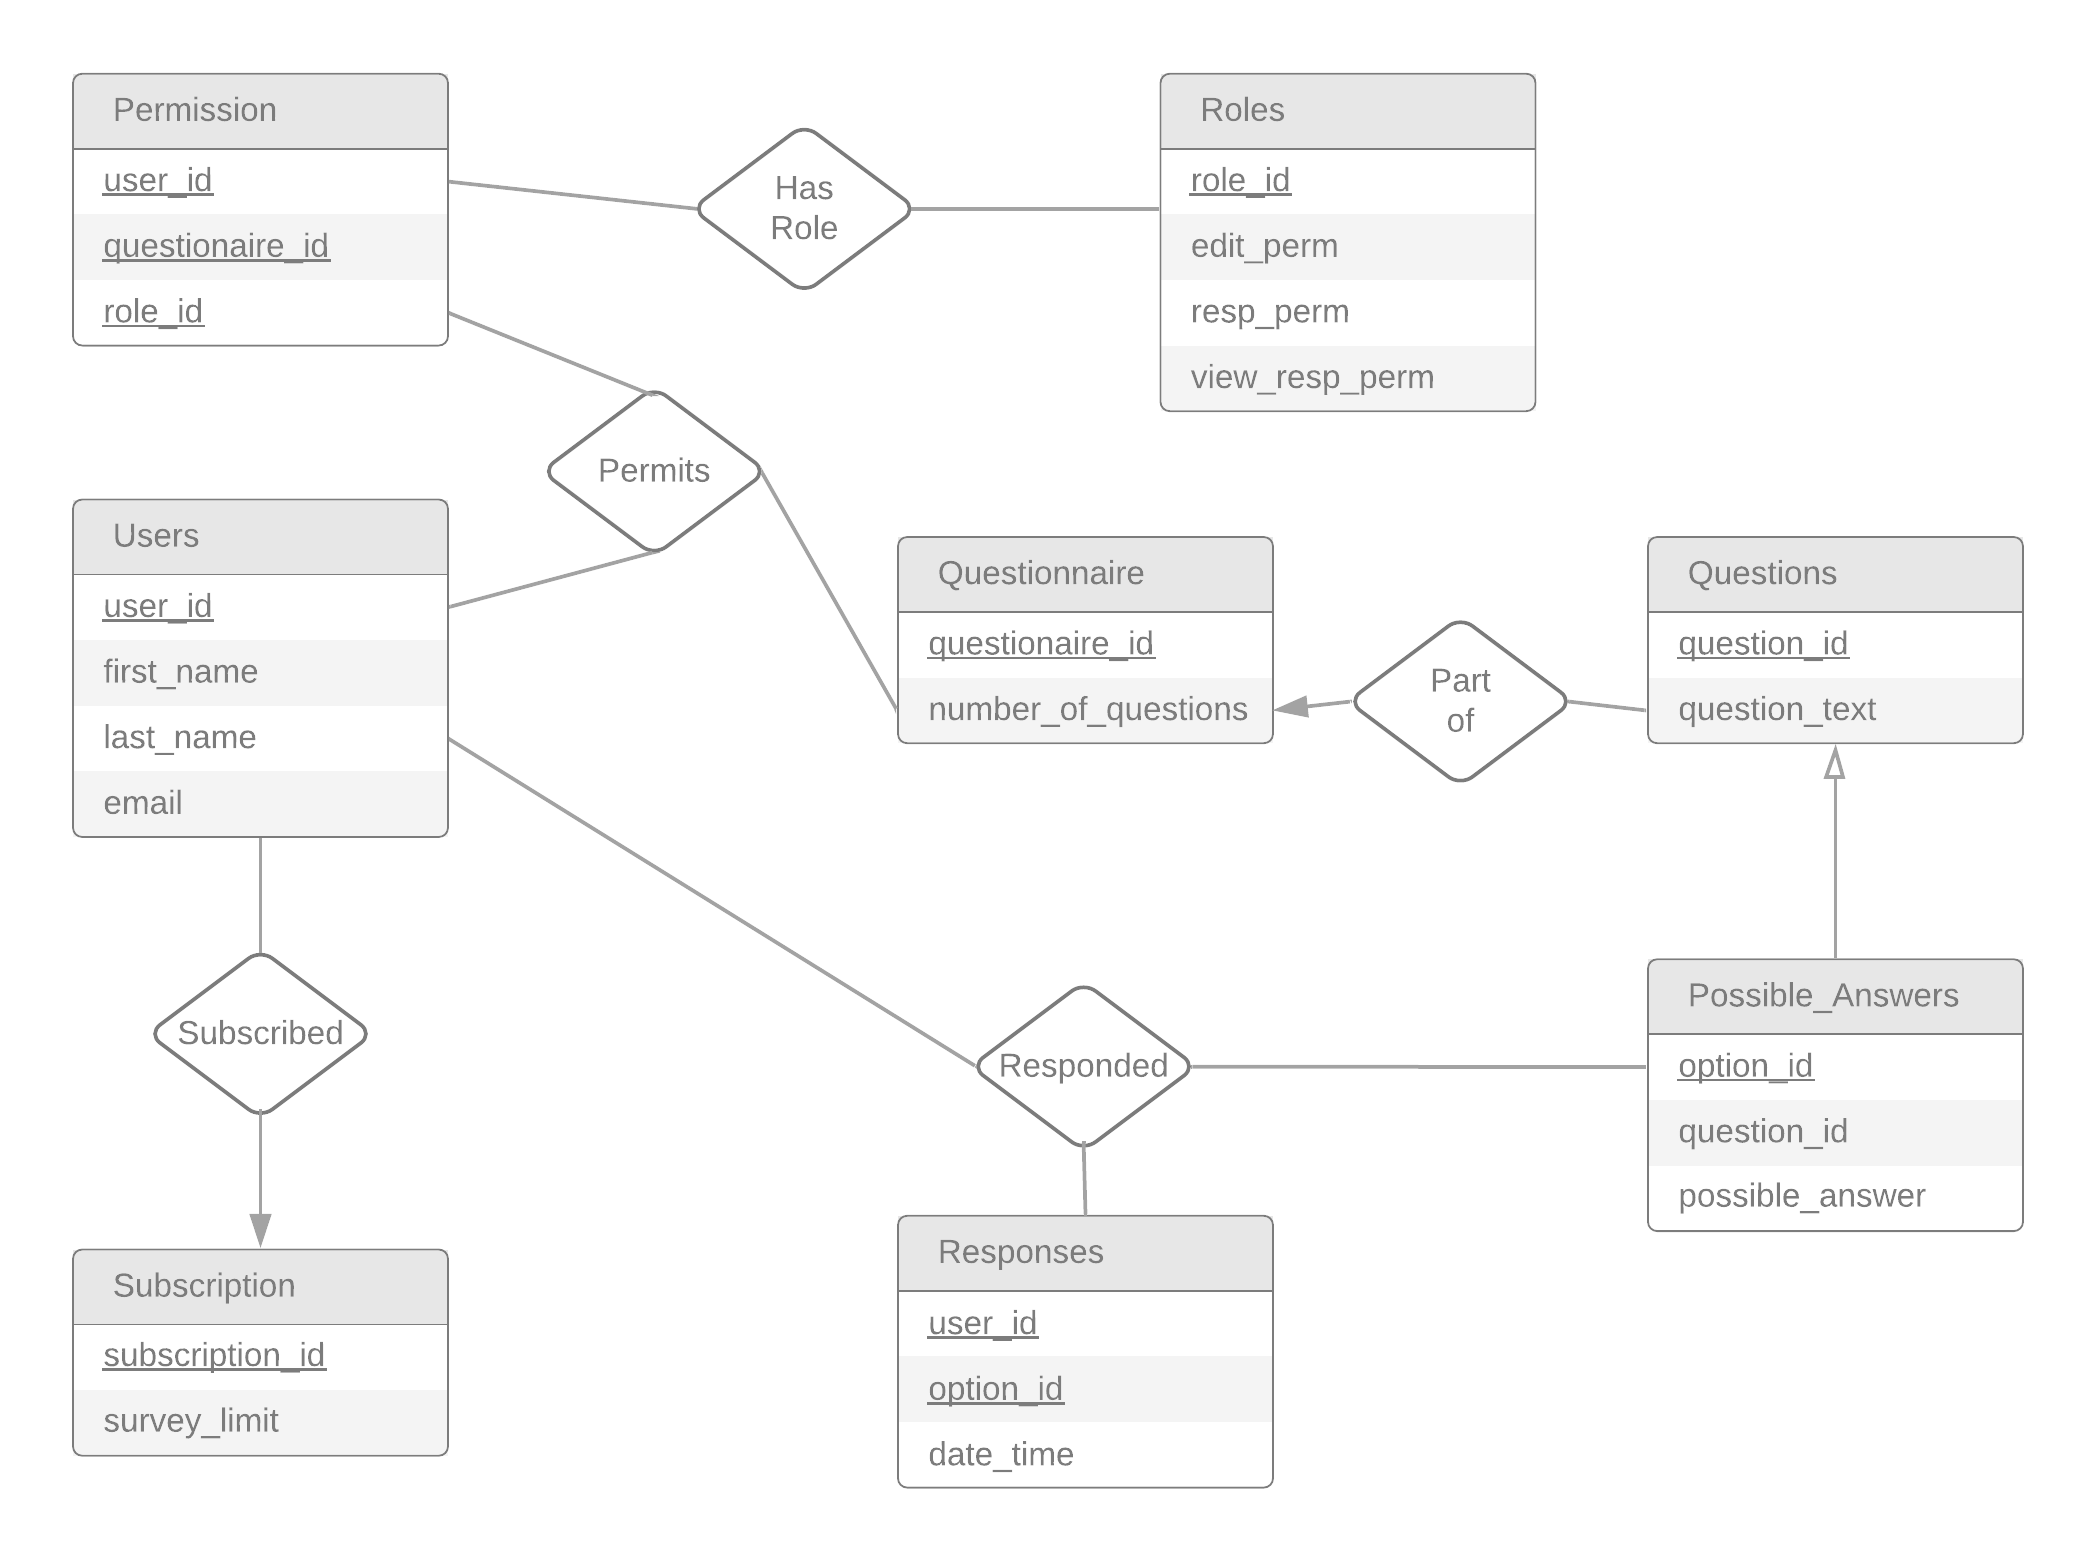
\includegraphics[width=\textwidth]{er_diagram.png}
        }
    \end{figure}
    

    \newpage
    \section{Data Description and Schemas}
    \begin{lstlisting}[language=SQL, columns=flexible]
        CREATE TABLE Users (
            user_id INT,
            first_name VARCHAR(40),
            last_name VARCHAR(40),
            email VARCHAR(100),
            subscription_id INT, 
            PRIMARY KEY(user_id),
            FOREIGN KEY(subscription_id REFERENCES Subscription(subscription_id))
        ) 
    \end{lstlisting}
    This entity represents users of the questionnaire website.
    All types of users, including people who create questionnaires
    or answer questionnaires, are in this table.
    \\

    \begin{lstlisting}[language=SQL, columns=flexible]
        CREATE TABLE Permissions (
            permission_id INT,
            user_id INT,
            questionnaire_id INT,
            role_id INT,
            PRIMARY KEY (permission_id),
            FOREIGN KEY(user_id REFERENCES Users(user_id)),
            FOREIGN KEY(questionnaire_id REFERENCES Questionnaires(questionnaire_id)),
            FOREIGN KEY(role_id REFERENCES Roles(role_id))
        ) 
    \end{lstlisting}
    This entity describes the permission level of a user for each 
    questionnaire, this is part of a ternary relationship between users, questionnaire, and permission. User and Questionnaire entities are not fully participating in this table. 
    \\
    
    \begin{lstlisting}[language=SQL, columns=flexible]
        CREATE TABLE Roles (
            role_id INT,
            edit_perm BIT, 
            resp_perm BIT,
            view_resp_perm BIT,
            PRIMARY KEY(role_id)
        ) 
    \end{lstlisting}
    This entity describes the roles that are allowed for each permission evel. For each role there are different permissions that are dependent on a true or false value (BIT) in SQL. For each tuple of user and survey the permission level determines what roles they have.
    \\

    \begin{lstlisting}[language=SQL, columns=flexible]
        CREATE TABLE Subscription (
            subscription_id INT,
            survey_limit INT, 
            PRIMARY KEY(subscription_id)
        ) 
    \end{lstlisting}
    Describes the subscription level and how many surveys users are allowed to create at each subscription level. 
    \\

    \begin{lstlisting}[language=SQL, columns=flexible]
        CREATE TABLE Questionnaires (
            questionnaire_id INT,
            number_of_questions INT, 
            PRIMARY KEY(questionnaire_id)
        ) 
    \end{lstlisting}
    Defines a questionnaire with the unique id that will be bound to a user using the permissions table. 
    \\

    \begin{lstlisting}[language=SQL, columns=flexible]
        CREATE TABLE Questions ( 
            question_id BIGINT,
            questionnaire_id INT,
            question_text VARCHAR(400), 
            PRIMARY KEY(question_id),
            FOREIGN KEY(questionnaire_id REFERENCES Questionnaires(questionnaire_id))
        ) 
    \end{lstlisting}
    Determines questions as they are related to each questionnaire. 
    \\

    \begin{lstlisting}[language=SQL, columns=flexible]
        CREATE TABLE Possible_Answers (
            option_id BIGINT,
            question_id BIGINT, 
            possible_answer VARCHAR(400),
            PRIMARY KEY(option_id),
            FOREIGN KEY(question_id REFERENCES Questions(question_id))
        ) 
    \end{lstlisting}
    Defines possible answers to each question. e.g. for multiple choice questions, this will have entries for each possible answer, while for questions like rating questions, this place will have the range of rankings available. 
    \\

    \begin{lstlisting}[language=SQL, columns=flexible]
        CREATE TABLE Responses (
            response_id INT,
            user_id INT,
            option_id BIGINT, 
            date_time DATETIME,
            PRIMARY KEY(response_id),
            FOREIGN KEY(user_id REFERENCES Users(user_id)), 
            FOREIGN KEY(option_id REFERENCES Possible_Answers(option_id))
        ) 
    \end{lstlisting}
    Defines the user response to each of the questions and ties them to the unique response option identifier and user id.
    \\

    Possible queries:   
    \begin{outline}
        \1 Check if user answered the survey
        \1 Check if user has permission to edit 
        \1 Check if user has permission to see analysis
        \1 Retrieve user answers
        \1 Retrive answer counts per question per questionnaire
        \1 Retrieve quetions related to questionnaire
        \1 Retrieve possible answers related to question
        \1 Distributions of responses to a question based on filters like date
        \1 Number of responses to a specific question
        \1 Query the number of times the question has been asked vs the response rate
        \1 Did person hit the limit of the number of questionnaires to create
    \end{outline}
    
    Improving performance:
    \begin{outline}
        \1 Create various table indexes
        \1 Create materialized views to improve performance on some of the queries
    \end{outline}
\end{document}